\documentclass[]{beamer}
%\documentclass[notes]{beamer}       % print frame + notes
%\documentclass[notes=only]{beamer}   % only notes
%\documentclass{beamer}              % only frames
%\documentclass[handout]{beamer}
\usepackage{amsmath}
\usepackage{tikz}
\usepackage{listings}

\usepackage{algorithm2e}

\usetheme{Dresden}%%%%% developer's preference - may change based on preferences

%%%%%% UMass official color: https://www.umass.edu/brand/elements/color
\definecolor{UMassAmherst}{rgb}{0.533 0.11 0.11}
\usecolortheme[named=UMassAmherst]{structure}

\title{Algoritmos}
\subtitle{Geometr\'ia Computacional}
\author{MSc Edson Ticona Zegarra}
\institute{Preparaci\'on ICPC Regionales}
\date{}
%\date{2023-I}

%%%%%% obtained from: https://www.umass.edu/brand/elements/wordmarks-seal-and-spirit-marks
%%%%%% logos of other departments can also be obtained from the above link. Otherwise, consult your department website.

%\titlegraphic{\includegraphics[width=0.5in]{logo_unmsm.png}}

\begin{document}

\maketitle

\begin{frame}{Contenido}
\tableofcontents
\end{frame}

\section{Puntos}
\begin{frame}{Puntos}
  \lstinputlisting[caption=Puntos en C++, label={lst:listing-cpp}, language=C++, basicstyle=\fontsize{8}{9}\selectfont]{points\_sample.cpp}
\end{frame}

\begin{frame}{Puntos}
  \lstinputlisting[caption=Puntos double, label={lst:listing-cpp}, language=C++, basicstyle=\fontsize{8}{9}\selectfont]{points\_double\_sample.cpp}
\end{frame}

\begin{frame}{Rotaci\'on}
  \begin{center}
    \begin{tikzpicture}[scale=2]
        % Draw axes
        \draw[->] (-1.5, 0) -- (1.5, 0) node[right] {$x$}; % X axis
        \draw[->] (0, -1.5) -- (0, 1.5) node[above] {$y$}; % Y axis

        % Original point
        \filldraw[red] (1, 0.5) circle (1pt) node[above right] {$P(x, y)$};

        % Rotated point
        \filldraw[blue] (0, 1.118) circle (1pt) node[above right] {$P'(x', y')$};

        % Draw angle arc
        \draw[thick, ->] (1, 0.5) arc[start angle=27, end angle=90, radius=1cm];
        \node at (0.7, 0.6) {$\theta$};

        % Dashed lines for reference
        \draw[dashed] (1, 0.5) -- (1, 0);
        \draw[dashed] (1, 0.5) -- (0, 0.5);
        \draw[dashed] (0, 1.118) -- (0, 0.5);
        \draw[dashed] (0, 1.118) -- (1, 0.5);
    \end{tikzpicture}
  \end{center}
\end{frame}

\begin{frame}{Matriz de rotaci\'on}
\[
\begin{bmatrix}
x' \\
y'
\end{bmatrix}
=
\begin{bmatrix}
\cos(\theta) & -\sin(\theta) \\
\sin(\theta) & \cos(\theta)
\end{bmatrix}
\begin{bmatrix}
x \\
y
\end{bmatrix}
\]
\end{frame}

\begin{frame}{Rotaci\'on}
  \lstinputlisting[caption=Rotaci\'on de puntos, label={lst:listing-cpp}, language=C++, basicstyle=\fontsize{8}{9}\selectfont]{point\_rotation.cpp}
\end{frame}

\section{Lineas}
\begin{frame}{Linea: $ax + by + c = 0$}
  \begin{center}
  \begin{tikzpicture}[scale=1.5]
      % Draw axes
      \draw[->] (-3, 0) -- (3, 0) node[right] {$x$}; % X axis
      \draw[->] (0, -2) -- (0, 3) node[above] {$y$}; % Y axis

      % Define the line ax + by + c = 0
      % Example line: 2x + y - 1 = 0 (a = 2, b = 1, c = -1)
      %\draw[thick, blue] (0.5, 0) -- (0, 1) node[below right] {$ax + by + c = 0$};
      \draw[thick, blue] (-1, 2.5) -- (2, -2) node[below right] {$ax + by + c = 0$};

      % Point at (-c/a, 0)
      \filldraw[red] (0.66, 0) circle (1pt) node[below right] {$(-\frac{c}{a}, 0)$};

      % Point at (0, -c/b)
      \filldraw[red] (0, 1) circle (1pt) node[above right] {$(0, -\frac{c}{b})$};

      % Dashed lines from the origin to the line showing intercepts
      \draw[dashed, gray] (0, 0) -- (0.5, 0);
      \draw[dashed, gray] (0, 0) -- (0, 1);

  \end{tikzpicture}
  \end{center}
\end{frame}

\begin{frame}{Lineas}
  \lstinputlisting[caption=Lineas en C++, label={lst:listing-cpp}, language=C++, basicstyle=\fontsize{8}{9}\selectfont]{lines\_sample.cpp}
\end{frame}

\begin{frame}{Vectores}
  \lstinputlisting[caption=Vectores, label={lst:listing-cpp}, language=C++, basicstyle=\fontsize{8}{9}\selectfont]{vectors\_sample.cpp}
\end{frame}

\begin{frame}{Producto punto}
\[
  \mathbf{a} \cdot \mathbf{b} = a_1 b_1 + a_2 b_2 + \cdots + a_n b_n = \sum_{i=1}^n a_i b_i
\]

\[
  \mathbf{a} \cdot \mathbf{b} = \|\mathbf{a}\| \|\mathbf{b}\| \cos \theta,
\]
\end{frame}

\begin{frame}{Producto cruz}
  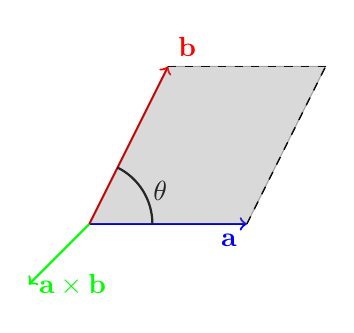
\begin{tikzpicture}
    % Define the vectors
    \coordinate (O) at (0,0,0);  % Origin
    \coordinate (A) at (2,0,0);  % Vector a
    \coordinate (B) at (1,2,0);  % Vector b
    \coordinate (AxB) at (0,0,2);  % Vector a x b

    % Draw the vectors
    \draw[thick,->,blue] (O) -- (A) node[anchor=north east] {$\mathbf{a}$};
    \draw[thick,->,red] (O) -- (B) node[anchor=south west] {$\mathbf{b}$};

    % Draw the parallelogram
    \draw[dashed] (A) -- ++(B) coordinate (AB);
    \draw[dashed] (B) -- ++(A);

    % Draw the cross product vector
    \draw[thick,->,green] (O) -- (AxB) node[anchor=west] {$\mathbf{a} \times \mathbf{b}$};

    % Draw the parallelogram (second set of vectors)
    \draw[dashed] (A) -- ++(B);
    \draw[dashed] (B) -- ++(A);

    % Draw angle arc
    \draw[thick] (0.8,0,0) arc[start angle=0,end angle=63.4349,radius=0.8] node[midway, right] {$\theta$};

    % Label the area
    %\node at (1.5,1,0) [anchor=south] {\text{Area} = $\|\mathbf{a} \times \mathbf{b}\| = \|\mathbf{a}\| \|\mathbf{b}\| \sin \theta$};

    % Draw the parallelogram's outline
    \draw[fill=gray,opacity=0.3] (O) -- (A) -- (AB) -- (B) -- cycle;
  \end{tikzpicture}
    Area = $\|\mathbf{a} \times \mathbf{b}\| = \|\mathbf{a}\| \|\mathbf{b}\| \sin \theta$
\end{frame}

\begin{frame}{Producto cruz}
\[
\mathbf{a} \times \mathbf{b} = \begin{vmatrix}
\mathbf{i} & \mathbf{j} & \mathbf{k} \\
a_1 & a_2 & a_3 \\
b_1 & b_2 & b_3
\end{vmatrix}
\]


\[
\mathbf{a} \times \mathbf{b} = (a_2 b_3 - a_3 b_2) \mathbf{i} - (a_1 b_3 - a_3 b_1) \mathbf{j} + (a_1 b_2 - a_2 b_1) \mathbf{k}.
\]

\end{frame}

\begin{frame}{Producto punto y cruz}
  \lstinputlisting[caption=Producto punto y cruz, label={lst:listing-cpp}, language=C++, basicstyle=\fontsize{8}{9}\selectfont]{vectors\_angle.cpp}
\end{frame}

\begin{frame}{CCW Test}
  \lstinputlisting[caption=Test CCW, label={lst:listing-cpp}, language=C++, basicstyle=\fontsize{8}{9}\selectfont]{vectors\_ccw.cpp}
\end{frame}

\section{Polygons}
\begin{frame}{Polygons}
  \begin{itemize}
    \item Representaci\'on can\'onica: lista de v\'ertices del pol\'igono en orden CW o CCW.
      \pause
    \item Se asume que el primer punto est\'a conectado con el \'ultimo punto
  \end{itemize}
\end{frame}

\begin{frame}{Per\'imetro}
  \lstinputlisting[caption=Per\'imetro del pol\'igono, label={lst:listing-cpp}, language=C++, basicstyle=\fontsize{8}{9}\selectfont]{polygons\_perimeter.cpp}
\end{frame}

\begin{frame}{\'Area}
\[
A = \frac{1}{2} \left| \sum_{i=1}^{n} (x_i y_{i+1} - y_i x_{i+1}) \right|
\]

  Donde A es el \'area de un pol\'igono definido por $n$ v\'ertices con coordenadas $(x_i, y_i)$, con $i=1, ..., n$
\end{frame}

\begin{frame}{\'Area}
  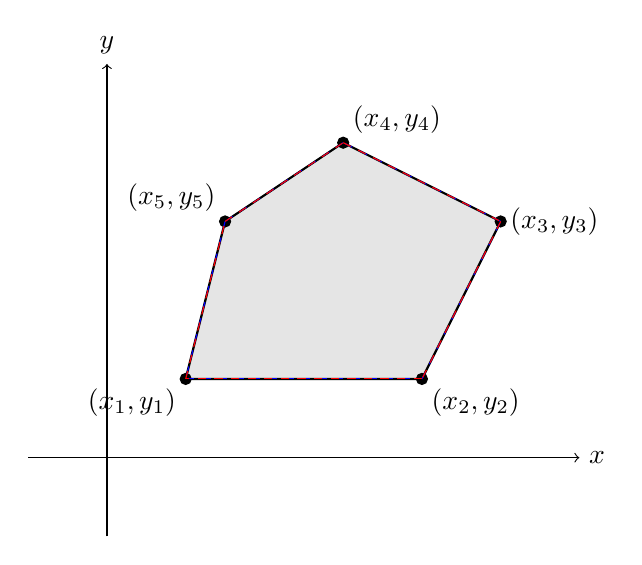
\begin{tikzpicture}
    % Define the coordinates of the polygon vertices
    \coordinate (A) at (1,1);
    \coordinate (B) at (4,1);
    \coordinate (C) at (5,3);
    \coordinate (D) at (3,4);
    \coordinate (E) at (1.5,3);

    % Draw the polygon
    \draw[thick, fill=gray!20] (A) -- (B) -- (C) -- (D) -- (E) -- cycle;

    % Draw the coordinate axes
    \draw[->] (-1,0) -- (6,0) node[right] {$x$};
    \draw[->] (0,-1) -- (0,5) node[above] {$y$};

    % Label the vertices
    \node[below left] at (A) {$(x_1, y_1)$};
    \node[below right] at (B) {$(x_2, y_2)$};
    \node[right] at (C) {$(x_3, y_3)$};
    \node[above right] at (D) {$(x_4, y_4)$};
    \node[above left] at (E) {$(x_5, y_5)$};

    % Draw the vertices
    \filldraw (A) circle (2pt);
    \filldraw (B) circle (2pt);
    \filldraw (C) circle (2pt);
    \filldraw (D) circle (2pt);
    \filldraw (E) circle (2pt);

    % Draw dashed lines to illustrate the shoelace pattern
    \draw[dashed, blue] (A) -- (B);
    \draw[dashed, blue] (B) -- (C);
    \draw[dashed, blue] (C) -- (D);
    \draw[dashed, blue] (D) -- (E);
    \draw[dashed, blue] (E) -- (A);

    \draw[dashed, red] (B) -- (A);
    \draw[dashed, red] (C) -- (B);
    \draw[dashed, red] (D) -- (C);
    \draw[dashed, red] (E) -- (D);
    \draw[dashed, red] (A) -- (E);

    % Add a legend for the summation
    % \node at (7,3) {
    % \begin{tabular}{c}
    % $\text{Area} = \frac{1}{2} \left| \sum (x_i y_{i+1} - y_i x_{i+1}) \right|$ \\
    % \small \text{where } $(x_{n+1}, y_{n+1}) = (x_1, y_1)$
    % \end{tabular}
    % };

  \end{tikzpicture}
\end{frame}

\begin{frame}{\'Area}
  \lstinputlisting[caption=\'Area del pol\'igono, label={lst:listing-cpp}, language=C++, basicstyle=\fontsize{8}{9}\selectfont]{polygons\_area.cpp}
\end{frame}

\begin{frame}{Convexidad}
  \begin{itemize}
    \item Se dice que un pol\'igono es convexo si para todo segmento formado por dos puntos interiores cualesquiera, el segmento es tambi\'en interno al pol\'igono
      \pause
    \item Un pol\'igono puede ser c\'oncavo o convexo
      \pause
    \item Los pol\'igonos convexos tienen propiedades interesantes y son ampliamente estudiantes en diversas \'areas
  \end{itemize}
\end{frame}

\begin{frame}{Convexidad}
  \lstinputlisting[caption=Test de convexidad, label={lst:listing-cpp}, language=C++, basicstyle=\fontsize{8}{9}\selectfont]{polygons\_convex.cpp}
\end{frame}

\end{document}
